\section{Performance evaluation}\label{sec:performance-evaluation}

To establish which method is better we can:
\begin{myitem}
    \item compare a single number,
    \item compare curves.
\end{myitem}

The recognition algorithm identifies (\textit{classifies}) the gallery image as matching the query object (test image) if their distance is below a threshold $t$. We can compare actual outcomes to predicted outcomes using a \textbf{confusion matrix} (\textit{classification matrix}):
\begin{table}[!h]
    \centering
    \begin{tabular}{l|l|l|}
        \cline{2-3}
        & Predicted = 0        & Predicted = 1    \\ \hline
        \multicolumn{1}{|l|}{Actual = 0}     & True Positives (TN)  & False Positives (FP) \\ \hline
        \multicolumn{1}{|l|}{Not Retrieved} & False Negatives (FN) & True Negatives (TN)  \\ \hline
    \end{tabular}
    \caption{Confusion matrix}
    \label{tab:confusion-matrix}
\end{table}

The higher the $t$, the more gallery images are classified as matching (more TP but also more FP); the smaller the t the less gallery images are classified as matching (more TN but also more FN).


\subsection{Single number evaluation metrics}\label{sec:pe-single}

$N = $ number of observations

\begin{myitem}
    \item \textbf{Overall accuracy}: How often the correct outcome is being predicted. How well a binary classification test correctly identifies or excludes a condition.
    \begin{equation}\label{eq:accuracy}
        ACC = \frac{TP+TN}{N}
    \end{equation}
    %
    \item \textbf{Overall error rate}:
    \begin{equation}\label{eq:error-rate}
        PPV = \frac{FP+FN}{N}
    \end{equation}
    %
    \item \textbf{Precision} (aka \textbf{Positive Predictive Value}): The fraction of relevant instances among the retrieved instances.
    (see figure \ref{fig:precision-recall})
    \begin{equation}\label{eq:precision}
        PPV = \frac{TP}{TP+FP}
    \end{equation}
    %
    \item \textbf{Recall} (aka \textbf{Sensitivity} or \textbf{True Positive Rate}): The fraction of relevant instances that have been retrieved over the total amount of relevant instances. The proportion of actual positives that are correctly identified as such.
    (see figure \ref{fig:precision-recall} and figure \ref{fig:sensitivity-specificity})
    \begin{equation}\label{eq:recall}
        TPR = \frac{TP}{TP+FN}
    \end{equation}
    %
    \item \textbf{Specificity} (aka \textbf{True Negative Rate}): The proportion of actual negatives that are correctly identified as such.
    (see figure \ref{fig:sensitivity-specificity})
    \begin{equation}\label{eq:specificity}
        TNR = \frac{TN}{FP+TN}
    \end{equation}
    %
    \item \textbf{Negative Predictive Value}: The proportions of negative results that are true negative results.
    \begin{equation}\label{eq:npv}
        NPV = \frac{TN}{TN+FN}
    \end{equation}
    %
    \item \textbf{Fall-out} (\textbf{False Positive Rate}):
    \begin{equation}\label{eq:fpr}
    FPR = 1-TNR = \frac{FP}{FP + TN}
    \end{equation}
    %
    \item \textbf{Miss rate} (\textbf{False Negative Rate}):
    \begin{equation}\label{eq:fnr}
    FNR=1-TPR
    \end{equation}
    %
    \item \textbf{False Discovery Rate}:
    \begin{equation}\label{eq:fdr}
        FDR=1-PPV
    \end{equation}
\end{myitem}

\begin{minipage}{.5\linewidth}
\begin{figure}[H]
    \centering
    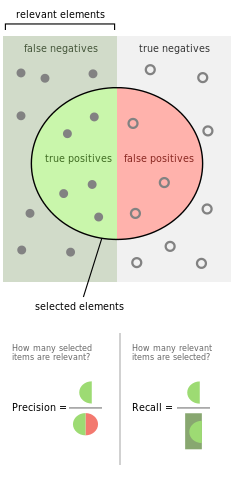
\includegraphics[width=.7\textwidth]{precision-recall}
    \caption[Precision-Recall]{Precision-Recall}
    \label{fig:precision-recall}
\end{figure}
\end{minipage}
\begin{minipage}{.5\linewidth}
\begin{figure}[H]
    \centering
    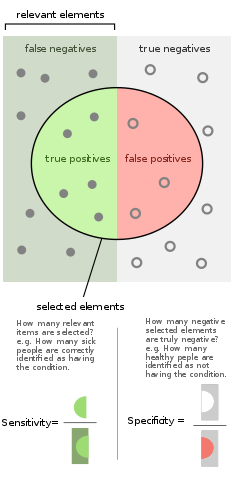
\includegraphics[width=.7\textwidth]{sensitivity-specificity}
    \caption[Sensitivity-Specificity]{Sensitivity-Specificity}
    \label{fig:sensitivity-specificity}
\end{figure}
\end{minipage}


\subsection{Curve-based metrics}\label{sec:ep-curves}

We can use curve-based metrics to find the best trade-off for the threshold value, balancing the cost of failing to identify an object and the cost of raising false alarms, depending on the task :
\begin{myitem}
    \item \textbf{Receiver Operating Curve}: It's a probability curve, the plot of the TPR against the FPR for a binary classification problem as you change the threshold. (see figure \ref{fig:roc-auc})
    %
    \item \textbf{Area under the Receiver Operating Curve (AUC)}: It represents degree or measure of separability, it tells us how much the model is capable of distinguishing between classes, i.e., the closer the AUC is to 1, better the model is at predicting 0s as 0s and 1s as 1s, the closer it is to 0.5, the more the model is similar to a random guess. AUC is less affected by sample balance than accuracy. (see figure \ref{fig:roc-auc})
    %
    \item \textbf{Precision-recall curve}: Preferred for detection, where TN's are undefined. (see figure \ref{fig:precision-recall-curve})
\end{myitem}

\begin{minipage}{.5\linewidth}
    \begin{figure}[H]
        \centering
        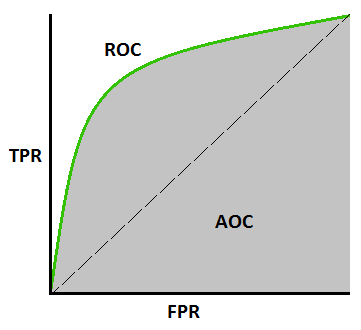
\includegraphics[width=.8\textwidth]{roc-auc}
        \caption[ROC-AUC curves]{ROC-AUC curves}
        \label{fig:roc-auc}
    \end{figure}
\end{minipage}
\begin{minipage}{.5\linewidth}
    \begin{figure}[H]
        \centering
        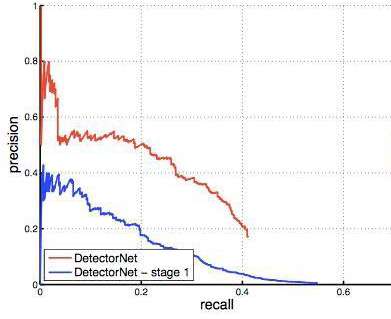
\includegraphics[width=.8\textwidth]{prc}
        \caption[Precision recall curve]{Precision recall curve}
        \label{fig:precision-recall-curve}
    \end{figure}
\end{minipage}
